\documentclass[draft,a4paper,english]{lipics-v2018}
\usepackage{microtype,amssymb,amsmath,stmaryrd,mathpartir,array,graphicx}%if unwanted, comment out or use option "draft"
\usepackage[table]{xcolor}
\newcommand{\xt}[1]{\texttt{#1}}
\newcommand{\tupleo}[1]{\xt{Tuple1\{}#1\xt{\}}}
\newcommand{\tuplet}[2]{\xt{Tuple2\{}#1,#2\xt{\}}}
\newcommand{\union}[2]{\xt{Union\{}#1,#2\xt{\}}}
\newcommand{\denotes}[1]{\llbracket #1 \rrbracket}

%FZ
\newcommand{\sub}{<:}
\newcommand{\tuple}[1]{\xt{Tuple\{}#1\xt{\}}}
\newcommand{\arrayt}[1]{\xt{Array\{}#1\xt{\}}}
%end FZ

\newcommand{\bsub}{<:_b}
\newcommand{\nsub}{<:_n}

\newcommand{\goodcell}{\cellcolor{green!25}}
\newcommand{\badcell}{\cellcolor{red!25}}

%\graphicspath{{./graphics/}}%helpful if your graphic files are in another directory

\bibliographystyle{plainurl}% the recommnded bibstyle

\title{On Julia's efficient algorithm for subtyping union types and covariant tuples (Pearl)}

%\titlerunning{Temporary Title}%optional, please use if title is longer than one line

\author{Anon}{None}{}{}{}

%\author{Benjamin Chung}{Northeastern University}{bchung@ccs.neu.edu}{}{}%mandato
%\author{Francesco Zappa Nardelli}{Inria}{}{}{}
%\author{Jan Vitek}{Northeastern University \& Czech Technical University}{}{}{}

\authorrunning{Anon}%B. Chung, F. Zappa Nardelli, J. Vitek}%mandatory. First: Use abb

\Copyright{Anon}%Benjamin Chung, Francesco Zappa Nardelli, Jan Vitek}%mandatory, plea

\subjclass{Dummy classification}% mandatory: Please choose ACM 2012 classifications from https://www.acm.org/publications/class-2012 or https://dl.acm.org/ccs/ccs_flat.cfm . E.g., cite as "General and reference $\rightarrow$ General literature" or \ccsdesc[100]{General and reference~General literature}. 

\keywords{Type systems, Subtyping, Union types}

\category{}%optional, e.g. invited paper

\relatedversion{}%optional, e.g. full version hosted on arXiv, HAL, or other respository/website

\supplement{}%optional, e.g. related research data, source code, ... hosted on a repository like zenodo, figshare, GitHub, ...

\funding{}%optional, to capture a funding statement, which applies to all authors. Please enter author specific funding statements as fifth argument of the \author macro.

% put the algorithm up front and explanation
% here's a cute and simple algorithm that works for distributive tuples and unions
% write it with imperative stacks
% tuple union is hard known for 20yrs sol w/ normalization
% prob 1: state explosion (also seen in swift) CDeuce approach doesn't work
% prob 2: expressivity interacting with rhicher type system normalization doesn't work at all
% what we show is an alternative way to deal with distributive subtyping
% sol prob 1: lazy stack-based subtyping algorithm
% sol prob 2: ....
%
\acknowledgements{}%optional

%Editor-only macros:: begin (do not touch as author)%%%%%%%%%%%%%%%%%%%%%%%%%%%%%%%%%%
\EventEditors{John Q. Open and Joan R. Access}
\EventNoEds{2}
\EventLongTitle{42nd Conference on Very Important Topics (CVIT 2016)}
\EventShortTitle{CVIT 2016}
\EventAcronym{CVIT}
\EventYear{2016}
\EventDate{December 24--27, 2016}
\EventLocation{Little Whinging, United Kingdom}
\EventLogo{}
\SeriesVolume{42}
\ArticleNo{23}
%\nolinenumbers %uncomment to disable line numbering
%\hideLIPIcs  %uncomment to remove references to LIPIcs series (logo, DOI, ...), e.g. when preparing a pre-final version to be uploaded to arXiv or another public repository
%%%%%%%%%%%%%%%%%%%%%%%%%%%%%%%%%%%%%%%%%%%%%%%%%%%%%%

\begin{document}

\maketitle
\begin{abstract}
  We describe the clever algorithm implemented in the Julia
  programming language runtime to decide subtype on a simple type
  system with union types, covariant tuples, and literals.  This
  algorithm is immune from the space-explosion and expressiveness
  problems of the standard algorithms based on normalising types in
  disjuntcive normal form ahead-of-time.  We additionally prove it
  correct and complete against a semantic-subtyping denotational model
  in Coq.
%%   Deciding subtype on Union types and covariant tuples present several

%%   We present the clever algorithm implemented in the Julia programming
%%   language to decide subtype on a core 
%% We describe a novel algorithm for deciding subtyping for a type language consisting
%% of tuples, unions, and existential type variables without normalization and requiring
%% space linear in the size of the input types. We prove algorithmic correctness with 
%% respect to a semantic notion of subtyping using a proof assistant. Finally, we examine
%% the algorithm's use in the Julia programming language.
\end{abstract}

\section{FZN Introduction}
%%% Please do not edit from here...

Union types are increasingly common in mainstream languages.
In some cases, as Julia~\cite{BezansonEKS17} or TypeScript~\cite{},
they are exposed at the source level. In others, as Hack~\cite{}, they
are only used internally when performing type inference; in all cases
they play a key role in the expressiveness of the language.

Rules for subtyping union types have been known for a long time, and
following Vouillon~\cite{Vouillon04} they may be written as:
\begin{mathpar}
\inferrule{t_1 \sub t \\ t_2 \sub t}{\union{t_1}{t_2} \sub t}

\quad

\inferrule{t \sub t_1}{t \sub \union{t_1}{t_2}}

\inferrule{t \sub t_2}{t \sub \union{t_1}{t_2}}
\end{mathpar}
It has also been known for a long time that, in presence of covariant
tuples, the above rules are not complete with respect to a semantic
subtyping model~\cite{}. In such a semantic model, covariant types
should be \emph{distributive} with respect to unions; under a distributive
system, the following derivation should hold:
\[
\tuple{\union{t_1}{t_2}, t} \ \ \sub\ \ \union{\tuple{t_1, t}}{\tuple{t_2, t}} 
\]
Recall the subtype rule for covariant tuples:
\[
\inferrule{t_1 \sub t'_1 \\ t_2 \sub t'_2}{\tuple{t_1, t_2} \sub \tuple{t'_1, t'_2}}
\]
With this rule, derivations must immediately pick either the left or
right component of the union type; as a result, it is impossible to 
conclude the above subtyping relation. The standard approach
to solve this conundrum is to rewrite all types into their
disjunctive normal form (DNF, unions of union-free types)
\emph{before} building the derivation. This rewriting step can be
implemented easily and its correctness can be justified by a
semantic-subtyping denotational model, as in~\cite{Frisch08}. Moreover, the
resulting subtype algorithm can be proved correct and
complete. However, the standard algorithm based on ahead-of-time
normalization has \emph{two major drawbacks}.  The first drawback is
that the normalization phase rewrites types into potentially
\emph{exponentially bigger} types. By instrumenting Julia's 
subtyping decision procedure when executing library code, we often observe queries
involving types as the one below:
\begin{small}
\begin{verbatim}
   Tuple{Tuple{Union{Int64, Bool}, Union{String, Bool}, Union{String, Bool}, 
               Union{String, Bool}, Union{Int64, Bool}, Union{String, Bool}, 
               Union{String, Bool}, Union{String, Bool}, Union{String, Bool}, 
               Union{String, Bool}, Union{String, Bool}, Union{String, Bool}, 
               Union{String, Bool}, Union{String, Bool}, Union{String, Bool}}, Int64}
 \end{verbatim}
\end{small}

Normalizing this type before attempting to decide subtyping is not a
realistic option, and solving a query where it is matched against a
type as 
\begin{small}
\begin{verbatim}
Tuple{Tuple{Any, Any, Any, Any, Any, Any, Any, Any, Any, Any, Any,
            Any, Any, Any, Any}, Any}
\end{verbatim}
\end{small}
(where \verb+Any+ is the supertype of all types) ought to be performed in
linear time.

The second drawback of ahead-of-time normalisation phase is that it does
not interact nicely with other type system features. Invariant
constructors make lifting all union types to the top level unsound.
Consider the type \(\arrayt{\union{t_1}{t_2}}\). It denotes the set 
of arrays whose elements are either of type \(t_1\) or \(t_2\). It 
would be incorrect to rewrite it as \(\union{\arrayt{t_1}} {\arrayt{t_2}}\), 
as this latter type denotes the set of arrays whose elements are either 
all of type \(t_1\) or all of type \(t_2\). A weaker normal form that
only lifts union types inside each invariant constructor might be able
to circumvent this problem, but this only reveals a deeper
problem in the presence of both invariant constructors and existential
types.
%\textbf{would be good to have one example of a language that
%    has both here}.
With such a weaker normal form, the judgment below should hold:
\[
  \arrayt{\union{\tuple{t_1}}{\tuple{t_2}}} \ \ <:\ \ \exists T\,.\, \arrayt{\tuple{T}}
\]
All types are in normal form, and a standard algorithm would initially
perform the left-to-right subtype check due to the outer invariant
constructor. In doing so, it would generate the constraint \(T\ >:\ \union{t_1}{t_2}\).
As a consequence, the subsequent right-to-left check
\(\tuple{T}\ \ <:\ \ \union{\tuple{t_1}\tuple{t_2}}\) gets stuck when trying
to prove \(T\ <:\ t_1\) or \(T\ <:\ t_2\). 

The key to derive a successful judgment for this relation is to rewrite the
right-to-left check into \(\tuple{T}\ \ <:\ \ \tuple{\union{t_1}{t_2}}\),
which is provable. This is a sort of \emph{anti-normalisation} rewriting, that
must be performed on sub-judgments of the derivation.

In this \emph{pearl paper} we describe how the clever algorithm used by
the Julia language to decide subtype computes subtyping in a core
language with only union types, covariant tuples, and literals, and we
will provide evidence that it does not suffer from the two drawbacks
above.  Our goal is to make this technique known to a wider audience,
as we expect that it lifts smoothly to other richer type systems as it
lifts smoothly to the full Julia type system.  Additionally we prove
in Coq that the algorithm is correct and complete with respect to a
standard semantics subtyping model.

\newpage

%Subtyping union types has been known for a long time.  Recall the rules.

%If we add covariant tuples, again, distributivity has been known for a
%long time.  Show the problem with standard rules.

%The standard solution is to rewrite types in normal form.  Explain normal form.

%This has two inconvenients:
%\begin{itemize}
%\item Space explosion.

  %\item Lack of completeness in presence of more expressive types,
%    eg.\ existential (explain Julia counterexample).
%\end{itemize}
%
%While subtyping union types is inherently exponential in time, it does
%not have to suffer from the above limitation wrt.\ space and
%expressiveness.
%%% ...to here
%%% END FZN Introduction    

\section{Prior Work}

Previous efforts to provide a decision procedure for distributive unions rely
heavily on normalization. In order to decide subtyping in one of these
approaches, the type is first normalized (to integrate the distributivity
axiom) and then the standard syntax-directed subtyping algorithm is applied to
conclude the subtyping
relation~\cite{muehlboeck2018empowering,Reynolds1997,Pierce1991}. This
normalization step puts the type into disjunctive normal form thereby allowing
the algorithmic union rule to decide subtyping correctly. As there are
exponentially many choice sets for any given type (where one of two choices
may be given at each union), the space taken up by the fully normalized type
can be substantial. Moreover, (in languages with some kind of higher-rank
polymorphism) the normalization process eliminates all internal unions; as a
concequence, variable instantiations may be over-specialized and some
semantically-valid subtyping relations may not hold.



\section{Algorithm}

Our algorithm for deciding subtyping works by iterating through every possible
choice that could be made between at branches of unions within the two types
participating in a subtype check. In this section, we will describe the
implementation of the algorithm in OCaml and will present our proof of
correctness in the following section.

The type language for our algorithm is a subset of that used in the Julia
programming language, removing type variables. So as to avoid needing an
additional externally-provided subtype hierarchy, we specify that atomic types
(atoms) are subtypes only if they are exactly the same.

\hspace{1em}

\begin{minipage}{\textwidth}
\begin{minipage}{0.4\textwidth}
\begin{verbatim}
type typ =
  | Atom of int
  | Tuple1 of typ
  | Tuple2 of typ * typ
  | Union of typ * typ

type st_choice = Left | Right
\end{verbatim}
\end{minipage}
\begin{minipage}{0.5\textwidth}
\begin{verbatim}
let rec initial_choice (a:typ) =
  match a with
  | Atom i -> []
  | Tuple1 t -> initial_choice t
  | Tuple2(t1,t2) -> (initial_choice t1) 
  		@ (initial_choice t2)
  | Union(l,r) -> Left::(initial_choice l)
\end{verbatim}
\end{minipage}
\end{minipage}
\hspace{1em}

\noindent The key construct for our algorithm is the \verb|st_choice|
operation, which represents whether the algorithm takes the left or the right
branch of a union. The algorithm stores the choice made at each union at the
present iteration in two stacks of \verb|st_choice|s, one for each side of the
subtype relation. 

To move through all possible choices, the \verb|next_state| function steps a
stack of \verb|st_choice|s to the next state. Here, we arbitrarily define next
state as ``the deepest unexplored alternative,'' or, equivalently, where the
last left has been converted to a right. We implement \verb|next_state| in two
distinct helper functions, the first of which implements the last-left-to-
right operation and the second implements a fix-up operation.

\begin{figure}
\begin{tabular}{cccc}
& \hspace{5em} & &\\
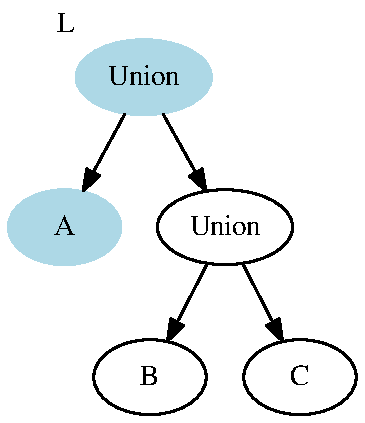
\includegraphics[scale=0.6]{figures-gen/example1.pdf} &
\multicolumn{2}{c}{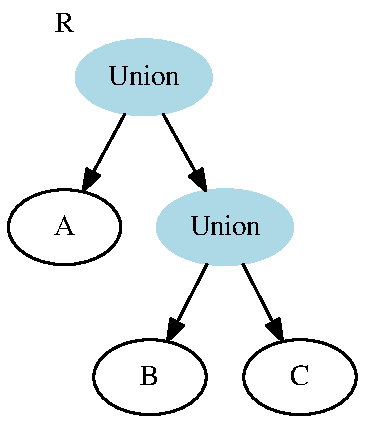
\includegraphics[scale=0.6]{figures-gen/example2.pdf}} &
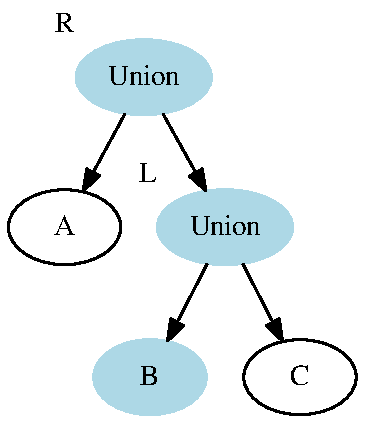
\includegraphics[scale=0.6]{figures-gen/example3.pdf} \\
L & \multicolumn{2}{c}{R} & RL \\
\multicolumn{2}{c}{last\_left\_to\_right} & \multicolumn{2}{c}{extend\_list} \\
\hline
\multicolumn{4}{c}{next\_state} \\
\end{tabular}
\caption{State-stepping operation for choice lists}
\label{fig:sstep}
\end{figure}

\begin{verbatim}
let rec last_left_to_right 
    (acc:st_choice list) (ll : st_choice list option) = function
  | Left::tl -> last_left_to_right (Left::acc) (Some (Right::acc)) tl
  | Right::tl -> last_left_to_right (Right::acc) ll tl
  | [] -> option_map List.rev ll
\end{verbatim}

The first step for the iteration function is \verb|last_left_to_right|. This
function finds the final Left instance in a list of choices and converts it to
a Right instance appended to the rest of the list unmodified. The new path
therefore points to the deepest as-yet unexplored path. However, its length
may be insufficient to  make a choice at each reachable union.

\begin{verbatim}
let rec extend_list (a:typ) (ls:st_choice list) = match (a,ls) with
  | (Atom i, _) -> ([], ls)
  | (Tuple1 t, _) -> extend_list t ls
  | (Tuple2(t1,t2), _) -> let (hd,tl) = extend_list t1 ls in
                          let (hd2,tl2) = extend_list t2 tl in
                          (hd @ hd2, tl2)
  | (Union(l,r), Left::rs) -> let (hd,tl) = extend_list l rs in (Left::hd,tl)
  | (Union(l,r), Right::rs) -> let (hd,tl) = extend_list r rs in (Right::hd,tl)
  | (Union(l,r), []) -> (Left::initial_choice l,[])
\end{verbatim}

\verb|extend_list| then finds where the new choice list runs out and fills it
out to be valid with respect to the type giving a valid state. If no successor
state is found---if there are no Left choices that remain---then the function
will return None.

\begin{verbatim}
let rec next_state (a:typ) (ls:st_choice list) =
  option_map fst (option_map (extend_list a) (last_left_to_right [] None ls))
\end{verbatim}

An example of a single step on the type $\union{A}{\union{B}{C}}$ is shown in
figure~\ref{fig:sstep}. Starting from the initial choice---simply picking the
left node---\verb|last_left_to_right| turns the left choice into a right choice.
This path is invalid for this type, however, so \verb|extend_list| is needed to
initialize the remainder of the path to make it valid. To do so, it picks the 
left choice at the terminal union, producing a valid path.

\begin{verbatim}
type st_res =
  | Subtype of st_choice list * st_choice list
  | NotSubtype
\end{verbatim}

\verb|st_res| represents the results of a single base subtype query. The query
can either succeed, in which case it provides the unused portion of the input
stacks, or fail. 

\begin{verbatim}
let rec base_subtype (a:typ) (b:typ) (fa:st_choice list) (ex : st_choice list)
  match (a,b,fa,ex) with
  | (Atom i, Atom j, _, _) -> if i == j then Subtype(fa, ex) else NotSubtype
  | (Tuple1 t1, Tuple1 t2, _, _) -> base_subtype t1 t2 fa ex
  | (Tuple2(ta1, ta2), Tuple2(tb1, tb2), _, _) ->
     (match base_subtype ta1 tb1 fa ex with
      | Subtype(cfa, cex) -> base_subtype ta2 tb2 cfa cex
      | NotSubtype -> NotSubtype)
  | (Union(a1,a2),b,choice::fa,ex) -> 
  		base_subtype (match choice with Left -> a1 | Right -> a2) b fa ex
  | (a,Union(b1,b2),fa,choice::ex) -> 
  		base_subtype a (match choice with Left -> b1 | Right -> b2) fa ex
\end{verbatim}

\verb|base_subtype| is responsible for using two paths---one for the left and
right hand sides of the subtyping relation---and checking that the subtype
relation holds with respect to those paths. Given a basic type---an atom or a
tuple---it will either check equality or recur respectively. Given a union, it
will grab the choice to make at that union off of the choice stacks and continue
recursively. The function then returns an instance of \verb|st_res|, which
gives the remaining choice stacks if successful or nothing otherwise.


\begin{figure}
\center
\begin{tabular}{cc|cc|c}
\multicolumn{2}{c}{Stack} & \multicolumn{2}{c}{Type} & Base Query \\
\hline
$\forall$ & $\exists$ & $\forall$ & $\exists$ & \\
\hline
\goodcell L & \goodcell L & \goodcell 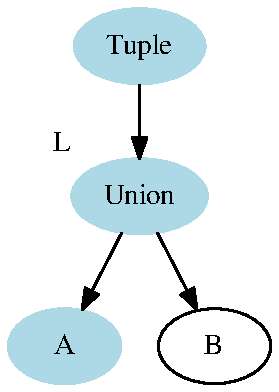
\includegraphics[scale=0.3]{figures-gen/left1.pdf} & \goodcell 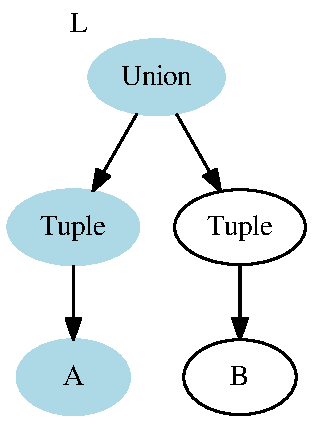
\includegraphics[scale=0.3]{figures-gen/right1.pdf} 
    & \goodcell $\tupleo{A} <: \tupleo{A}$ \\
\goodcell L & \badcell R & \badcell 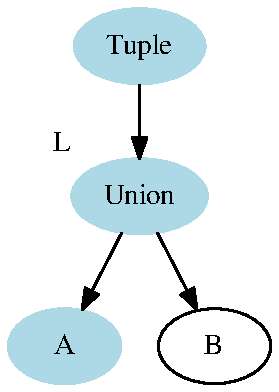
\includegraphics[scale=0.3]{figures-gen/left1.pdf} & \badcell 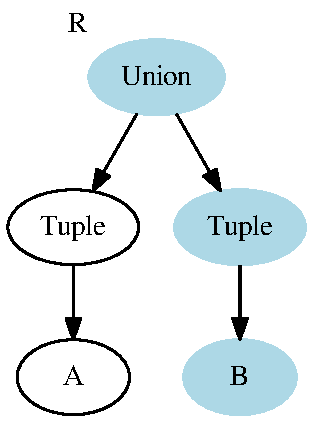
\includegraphics[scale=0.3]{figures-gen/right2.pdf}  
    & \badcell $\tupleo{A} \not<: \tupleo{B}$ \\
\hline
\goodcell R & \badcell L & \badcell 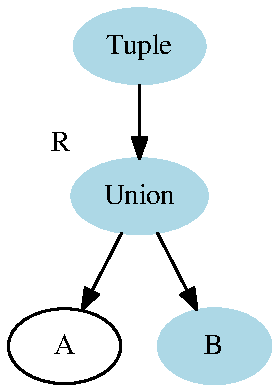
\includegraphics[scale=0.3]{figures-gen/left2.pdf} & \badcell 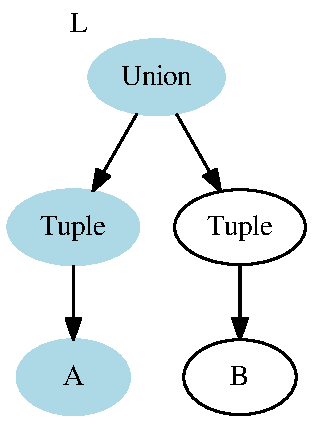
\includegraphics[scale=0.3]{figures-gen/right1.pdf}  
    & \badcell $\tupleo{B} \not<: \tupleo{A}$ \\
\goodcell R & \goodcell R & \goodcell 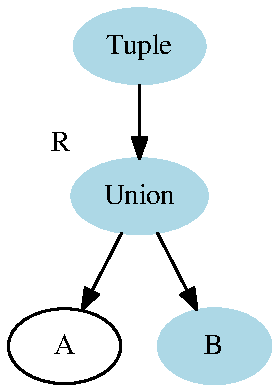
\includegraphics[scale=0.3]{figures-gen/left2.pdf} & \goodcell 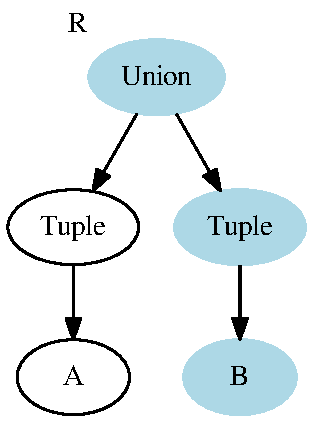
\includegraphics[scale=0.3]{figures-gen/right2.pdf}  
    & \goodcell $\tupleo{B} <: \tupleo{B}$ \\
\hline
\end{tabular}

\hspace{1em}

$\tupleo{\union{A}{B}} <: \union{\tupleo{A}}{\tupleo{B}}$

\caption{Subtyping decision procedure example}
\label{fig:cfs}
\end{figure}


Finally, to check subtyping, we need to iterate through both types in the 
correct quantification order. Subtyping holds if, for every instantiation 
of the left there exists an instantiation of the right hand side of the
subtyping judgment such that the subtype relation holds. To check this,
we use a simple brute force approach sitting atop the choice stack iterator
infrastructure described previously. The algorithm is implemented in two
functions. \verb|ex_subtype| checks that there exists an instantiation
of the right-hand-side for a given left-hand-side. \verb|fa_ex_subtype|
uses \verb|ex_subtype| to check that for every instantiation of the LHS,
there is an instantiation of the RHS such that the subtype relation holds.

\begin{verbatim}
let rec ex_subtype (a:typ)(b:typ)(fa:st_choice list)(cex : st_choice list) =
  match base_subtype a b fa cex with (* is a <: b *)
  | Subtype(_,_) -> true (* there exists a subtype *)
  | NotSubtype -> 
     (match next_state b cex with (* step exists-env *)
      | Some ns -> ex_subtype a b fa ns (* continue *)
      | None -> false) (* no subtype; exit *)

\end{verbatim}

If the current choice --- given by \verb|cex| --- is a supertype of the given \verb|a| according
to \verb|base_subtype|, then \verb|ex_subtype| has found a valid instantiation of \verb|b|. Therefore,
there exists an instantiation of \verb|b| that is a supertype of \verb|a| and the result should be true.
Otherwise, \verb|ex_subtype| will use the iteration operation, \verb|next_state|, to continue iterating
through choices for \verb|b| until it either finds an instantiation that is a supertype or runs out
of instantiations.

\begin{verbatim}
let rec fa_ex_subtype (a:typ)(b:typ)(cfa:st_choice list) =
  match ex_subtype a b cfa (initial_choice b) with (* a <: b wrt path? *)
  | true -> (match next_state a cfa with
               | Some ns -> fa_ex_subtype a b ns (* continue *)
               | None -> true) (* all subtypes; is subtype *)
  | false -> false (* exists a non-subtype; not subtype *)
\end{verbatim}

\verb|fa_ex_subtype| is very similar. It checks that for every
instantiation of \verb|a|, there exists an instantiation of 
\verb|b| such that subtyping holds. Checking for an instantiation
of \verb|b| is done using \verb|ex_subtype|, while \verb|fa_ex_subtype|
maintains an iterator for \verb|a|.

\begin{verbatim}
let rec subtype (a:typ) (b:typ) = fa_ex_subtype a b (initial_choice a)
\end{verbatim}

Finally, \verb|subtype| checks if \verb|a| is a subtype of \verb|b|.
It seeds \verb|fa_ex_subtype| with the initial choice for \verb|a|'s
iterator, which then checks if for every instantiation of \verb|a|
there exists an instantiation of \verb|b| such that subtyping holds.

Figure~\ref{fig:cfs} shows the execution of this function when checking the
relation $\tupleo{\union{A}{B}} <: \union{\tupleo{A}}{\tupleo{B}}$. For each
instantiation of the $\forall$ choice stack, there needs to be an
instantiation  of the $\exists$ stack such that when the type is subsetted
using those stacks the subtype relation holds.

\section{Proof}

To prove correctness of our algorithm, we begin by formally specifying
correctness for subtyping. We then show that three subtyping algorithms---
based on  normalization, structural iterators, and choice lists---are correct
with respect to this definition.

We base our definition of subtyping on a denotational semantics for types. 
We reduce types in the type language including unions to sets of types
in the type language without unions through a simple transformation. 

\begin{align*}
\denotes{\xt{A}} &= \{A\} \\
\denotes{\union{t_1}{t_2}} &= \denotes{t1} \cup \denotes{t2} \\
\denotes{\tupleo{t}} &= \{\tupleo{t'} | t' \in \denotes{t}\} \\
\denotes{\tuplet{t_1}{t_2}} &= \{\tuplet{t'_1}{t'_2} | t_1' \in \denotes{t_1},  t_2' \in \denotes{t_2'}\} \\
\end{align*}

Using this denotational semantics for types-with-unions, we can define
subtyping as $\denotes{t_1} \subseteq \denotes{t_2}$, then $t_1 <: t_2$.
Equivalently, we can state this as definition~\ref{dfn:scr}, which is canonicalized
in our Coq proof as the \verb|NormalSubtype| relation.

\begin{definition}[Subtyping Correctness]
A subtyping relation $<:$ is correct if $t_1 <: t_2$ iff $\forall t_1' \in \denotes{t_1},
\exists t_2' \in \denotes{t_2}, t_1 \bsub t_2$.
\label{dfn:scr}
\end{definition}

Proving a subtyping algorithm sound and complete is therefore equivalent to
producing a function of type \verb|forall t1 t2:type, {NormalSubtype t1 t2} + {~NormalSubtype t1 t2}|; that is, is able to decide whether two types are
subtypes or not.

\subsection{Normalization}

Following prior work, and to validate our definition, we first prove
equivalence of our definition to normalization-based subtyping. To do so, we
first define the normalization algorithm, then show that applying Vouillon-
style~\cite{Vouillon04} typing rules over the normalized types satisfies our
definition.

For this simple type language, normalization is equivalent to computing the
denotation set for the type. We define a metafunction \texttt{normalize}:

\[
\xt{normalize}(t) = \xt{Union}\{\denotes{t}\}
\]

For convenience of notation, we elide the nested unions that would be needed
if $|\denotes{t}| > 2$ and that if $|\denotes{t}| = 1$ then no union will be
generated. We can then define a correct semantic subtyping relation for our type
language using this metafunction. 

\begin{mathpar}
\inferrule{\xt{normalize}(t_1) \bsub \xt{normalize}(t_2)}{t_1 \nsub t_2}
\end{mathpar}

This normalization-based subtyping relation satisfies definition~\ref{dfn:scr}.

\begin{theorem}[Correctness of Normalization-Based Subtyping]
$t_1 \nsub t_2$ iff $\forall t_1' \in \denotes{t_1},
\exists t_2' \in \denotes{t_2}, t_1 \bsub t_2$
\end{theorem}
\begin{proof}
See the Coq implementation of \verb|normalize_subtype|. 
\end{proof}

We have proven that normalization combined with classical structural
type rules is equivalent to our denotational definition of subtyping.
However, as previously mentioned, normalization is slow, space intensive,
and precludes some algorithmic decisions on richer type languages. We therefore
will next discuss our iterator-based algorithm for deciding subtyping.

\subsection{Iterators}

The iterator-based implementation is directly equivalent (as will be shown
later) to the choice-stack based implementation presented previously in OCaml.
However, it retains type structure information inside of the iterator state.

\begin{verbatim}
Inductive TypeIterator: type -> Set :=
| TIAtom : forall i, TypeIterator (atom i)
| TITuple1 : forall tp, TypeIterator tp -> TypeIterator (tuple1 tp)
| TITuple2 : forall t1 t2, TypeIterator t1 -> TypeIterator t2 -> TypeIterator (tuple2 t1 t2)
| TIUnionL : forall t1 t2, TypeIterator t1 -> TypeIterator (union t1 t2)
| TIUnionR : forall t1 t2, TypeIterator t2 -> TypeIterator (union t1 t2).
\end{verbatim}

The \verb|TypeIterator| structure follows the structure of the type being
iterated over. Choices at unions are represented as either an instance of
\verb|TIUnionR| or \verb|TIUnionL|. This structure then lets us trivially
define a function that extracts the current type at the iterator's position:

\begin{verbatim}
Fixpoint current (t:type)(ti:TypeIterator t):type :=
match ti with
| TIAtom i => atom i
| TITuple1 tip p => tuple1 (current tip p)
| TITuple2 ti1 ti2 p1 p2 => tuple2 (current ti1 p1) (current ti2 p2)
| TIUnionL ti1 ti2 pl => (current ti1 pl)
| TIUnionR ti1 ti2 pr => (current ti2 pr)
end.
\end{verbatim}

Next, we can define a function that produces the initial iterator state for a
given type:

\begin{verbatim}
Fixpoint start_iterator (t:type):TypeIterator t :=
  match t with
  | (atom i) => TIAtom i
  | (tuple1 t) => TITuple1 t (start_iterator t)
  | (tuple2 t1 t2) => TITuple2 t1 t2 (start_iterator t1) (start_iterator t2)
  | (union t1 t2) => TIUnionL t1 t2 (start_iterator t1)
  end.
\end{verbatim}

Next, we can define a step function that takes one state and either steps it
to the next state or indicates that no such next state exists.

\begin{verbatim}
Fixpoint next_state (t:type)(ti:TypeIterator t) : option (TypeIterator t) :=
  match ti with
  | TIAtom i => None
  | TITuple1 tip p => option_map (TITuple1 tip) (next_state tip p)
  | TITuple2 ti1 ti2 p1 p2 =>
    match (next_state ti2 p2) with
    | Some np2 => Some(TITuple2 ti1 ti2 p1 np2)
    | None =>
      match (next_state ti1 p1) with
      | Some np1 => Some(TITuple2 ti1 ti2 np1 (start_iterator ti2))
      | None => None
      end
    end
  | TIUnionL ti1 ti2 pl =>
    match (next_state ti1 pl) with
    | Some npl => Some(TIUnionL ti1 ti2 npl)
    | None => Some(TIUnionR ti1 ti2 (start_iterator ti2))
    end
  | TIUnionR ti1 ti2 pr => option_map (TIUnionR ti1 ti2) (next_state ti2 pr)
  end.
\end{verbatim}

With these definitions, we can then prove a basic form of correctness with
respect to the denotational or normalization semantics:

\begin{theorem}[Correctness of iterators]
Every type in $\denotes{t}$ will be explored using \verb|next_step| from \verb|start_iterator t| 
\end{theorem}
\begin{proof}
See \verb|iterator_has_clauses| in the Coq proof.
\end{proof}

\verb|next_state| returns \verb|Some s| if there is some successor state
\verb|s| to the current, and \verb|None| if the given iterator state is
terminal. It will go left-to-right through unions, and will explore 2-tuples
by iterating through the choices on the right for each choice on the left. We can
then define an induction principle for type iterators based on \verb|next_state|:

\begin{theorem}
\begin{verbatim}
Definition iter_rect
  (t:type) (P:TypeIterator t -> Set)
           (pi: forall it, next_state t it = None -> P it)
           (ps : forall it' it'', P it'' -> next_state t it' = Some it'' -> P it')
           (it : TypeIterator t) : P it  
\end{verbatim}

For any type \verb|t| and proposition \verb|P|, and if:
\begin{itemize} 
	\item \verb|P| holds for an iterator that has no next state (e.g. is done)
	\item if \verb|P| holds for the \emph{following} iterator state \verb|it|,
	then \verb|P| holds for the \emph{preceeding} iterator state \verb|it'|.
\end{itemize}
Then \verb|P| holds for all iterators for type \verb|t|
\end{theorem}
\begin{proof}
See the Coq definition of \verb|iter_rect|.
\end{proof}

Using \verb|iter_rect|, we can implement and prove correct equivalent functions
to \verb|ex_subtype|, \verb|fa_ex_subtype|, and \verb|subtype| as described in the
OCaml implementation.

\begin{verbatim}
Definition exists_iter(a b : type) : 
  ({ t | InType t b /\ BaseSubtype a t } +
   {forall t, InType t b -> ~(BaseSubtype a t) }).
\end{verbatim}

\verb|exists_iter| is equivalent to the choice-stack based \verb|ex_subtype|,
and determines if there exists some denotationally-contained type in \verb|b|
that is a supertype of the given \verb|a|. Internally, it is implemented in 
the same way as \verb|ex_subtype|, though using \verb|iter_rect| to iterate 
through every iterator state.

\begin{verbatim}
Definition forall_iter (a b : type) :
  { forall t, In t (clauses a) -> exists t', InType t' b /\ (BaseSubtype t t')} +
  { exists t, In t (clauses a) /\ forall t', InType t' b -> ~ (BaseSubtype t t')}.
\end{verbatim}

\verb|forall_iter| is to \verb|fa_ex_subtype| what \verb|exists_iter| is to
\verb|ex_subtype|. Like \verb|exists_iter| it implements the same decision procedure
as \verb|fa_ex_subtype| (and internally relies upon \verb|exists_iter|), though through
the abstraction of \verb|iter_rect|.

Finally, we can define a decidable function (called \verb|subtype| in the proof)
that decides whether two types are subtypes or not. \verb|subtype| simply invokes
\verb|forall_iter| to decide subtyping.

\begin{verbatim}
Definition subtype(a b:type) : {NormalSubtype a b} + {~NormalSubtype a b}.
  destruct (forall_iter a b).
  - left. [...]
  - right. [...]
Defined.
\end{verbatim}

Therefore, using iterators, we can decide whether subtyping holds for any two types
in our language. We will now show an equivalence between iterators and stacks-of-choices,
allowing for more efficient implementation.

\subsection{Stacks}

To show that the choice-stack based algorithm is correct, we reduce it to the
already-shown-correct iterator-based algorithm for deciding subtyping. To do so,
we show an equivalence between choice stacks and iterators, then prove correctness
of the subtyping algorithms.

In the context of the Coq proof, we use the type \verb|st_context| to refer
to a choice stack. In Coq, this is represented as a list of boolean values,
with false representing a left choice and true representing a right choice at
a specific union.

To show equivalence between the iterator-based and stack-based algorithm, we need to
first prove two properties:

\begin{itemize}
  \item iterators are convertible to equivalent choice lists;
  \item stepping an iterator is equivalent to stepping a choice list.
\end{itemize}

We define an iterator and a choice stack to be equivalent if, when applied to
the same type, they select the same subset of that type. To describe this, we
define \verb|lookup_path| which looks up what type is selected by a given
choice stack.

\begin{verbatim}
Fixpoint lookup_path(t:type)(p:st_context) : type * st_context :=
  match t, p with
  | atom i, _ => (t, p)
  | tuple1 t, _ => let (r,p) := lookup_path t p in (tuple1 r, p)
  | tuple2 t1 t2, _ =>
    let (r1,p1) := lookup_path t1 p in
    let (r2,p2) := lookup_path t2 p1 in
    (tuple2 r1 r2, p2)
  | union l r, false::rs => lookup_path l rs
  | union l r, true::rs => lookup_path r rs
  | _, nil => (t, nil)
  end.
\end{verbatim}

\verb|lookup_path| is notable in that it both returns the selected type as
well as whatever of the choice stack remains once it reaches a leaf. This is
needed in order to be able to traverse types that contain tuples,  whose left
branches will potentially be given a longer choice stack then necessary.

Next, we can convert iterators to paths in the straightforward manner, as
implemented by \verb|iterator_to_path|:

\begin{verbatim}
Fixpoint iterator_to_path(t:type)(it:TypeIterator t):st_context :=
   match it with
   | TIAtom _ => nil
   | TITuple1 tp it1 => iterator_to_path tp it1
   | TITuple2 t1 t2 it1 it2 => (iterator_to_path t1 it1) ++ (iterator_to_path t2 it2)
   | TIUnionL t1 _ it1 => false :: (iterator_to_path t1 it1)
   | TIUnionR _ t2 it1 => true :: (iterator_to_path t2 it1)
   end.
\end{verbatim}

\verb|iterator_to_path| simply traverses the iterator in order, appending onto the
output choice stack whatever choice the iterator makes at that union. This illustrates
the equivalence between iterators and choice stacks; choice stacks are simply iterators
with the structural information removed.

Using the combination of \verb|lookup_path| and \verb|iterator_to_path|, we
can then show the first correctness property that we need to prove that the
algorithm using choice stacks is correct:

\begin{lemma}[Iterator to path is correct]
\begin{verbatim}
Lemma itp_correct : forall t it, current t it = fst (lookup_path t (iterator_to_path t it)).
\end{verbatim}

For every type \verb|t| and type iterator \verb|it|, the iterator's current type \verb|current t it| is equal
to the result of looking up the conversion of \verb|it| to a choice stack.
\end{lemma}
\begin{proof}
See \verb|itp_correct| in the Coq proof.
\end{proof}

Stepping in the Coq implementation is implemented identically to the OCaml
implementation. It only remains to show that this step operation (called
\verb|step_ctx| in Coq) is correct with respect to the iterator
\verb|next_state|.

\begin{lemma}[Correctness of step\_ctx]
\begin{verbatim}
forall t it,
    step_ctx t (iterator_to_path t it) =
    (option_map (iterator_to_path t) (next_state t it)).
\end{verbatim}
For every type \verb|t| and type iterator \verb|it|,
stepping the choice-list equivalent of \verb|it| will
produce the same result as converting the result of stepping
\verb|it|.
\end{lemma}
\begin{proof}
See \verb|list_step_correct| in the Coq proof.
\end{proof}

Now, with the relevant properties proven, we can implement and prove correct
\verb|ex_subtype| and \verb|fa_ex_subtype| in Coq. The function names are the
same, as are the implementations up to the addition of a fuel parameter (which
is shown to be unnecessary). 

\begin{lemma}[Correctness of existential subtype checking with choice stacks]
\begin{verbatim}
forall a b it, 
  (exists pf, exists_iter_inner a b it = inleft pf) <->
   exists n, ex_subtype a b (iterator_to_path b it) n = Some true.
\end{verbatim}
For every two types \verb|a| and \verb|b|, the iterator-based algorithm
\verb|exists_iter_inner| will produce a proof that \verb|a| is a subtype
of \verb|b| if and only if there is an integer \verb|n| such that
 \verb|ex_subtype| given \verb|n| fuel runs producing true.
\end{lemma}
\begin{proof}
See \verb|ex_sub_corr_eq| in the Coq proof.
\end{proof}

\begin{lemma}[Correctness of forall-exists subtype checking with choice stacks]
\begin{verbatim}
forall a b it,
   (exists pf, forall_iter_inner a b it = left pf) <->
    exists n, fa_ex_subtype a b (iterator_to_path a it) n = Some true.
\end{verbatim}
For every two types \verb|a| and \verb|b|, the iterator-based algorithm
\verb|forall_iter_inner| will produce a proof that \verb|a| is a subtype
of \verb|b| if and only if there is an integer \verb|n| such that
 \verb|fa_ex_subtype| given \verb|n| fuel runs producing true.
\end{lemma}
\begin{proof}
See \verb|fa_sub_corr_eq| in the Coq proof.
\end{proof}

The choice stack-based algorithm produces the same results as the 
iterator-based algorithm. 

%\bibliographystyle{plain}
\bibliography{refs}

\end{document}
